\documentclass{article}
\usepackage[spanish]{babel}
\usepackage[utf8]{inputenc}
\usepackage[nonatbib]{../template}

\usepackage[utf8]{inputenc} % allow utf-8 input
\usepackage[T1]{fontenc}    % use 8-bit T1 fonts
\usepackage{hyperref}       % hyperlinks
\usepackage{url}            % simple URL typesetting
\usepackage{booktabs}       % professional-quality tables
\usepackage{amsfonts}       % blackboard math symbols
\usepackage{nicefrac}       % compact symbols for 1/2, etc.
\usepackage{microtype}      % microtypography
\usepackage{xcolor}         % colors
\usepackage{graphicx}
\usepackage{float}
\usepackage[backend=biber,sorting=ynt,style=apa]{biblatex}

\addbibresource{../bibliography.bib}

\graphicspath{ {../imagenes/} }

\title{Entrega 3: Introducción y Resultados}

\author{%
  José Saint Germain\\
  \texttt{josesg998@gmail.com} \\
}

\begin{document}

\maketitle

% add TOC
\tableofcontents
\pagebreak

\section{Introducción}

% Explicar la merma de golpes de estado, en especial en LATAM

% Mencionar dos o tres autores que mencionen los motivadores de golpes

El objetivo de este trabajo es lograr entrenar un modelo de aprendizaje automático
que logre predecir de manera aceptable golpes de estados durante los años 2020 a 2022 
en todos los países del mundo a partir de la utilización de la base de datos provista 
por la fundación Varieties of Democracy (V-Dem) \cite{Cop24}, así como tener una noción 
acabada de la importancia de las distintas variables que componen esta base de datos para 
la correcta predicción de la variable objetivo. Para llevar a cabo este último objetivo 
se utilizaran tanto los mismos componentes de los algoritmos (importancia de atributos)
como la de los valores Shapley.

\subsection{Motivación}
% Motivación del paper (comparar con el poder predictivo de la base del FMI)
La motivación de este trabajo es dialogar con el artículo recientemente realizado por el 
Fondo Monetario Internacionl (FMI) \cite{Ceb24}. En el mismo se aborda  el mismo objeto 
de estudio utilizando diversas metodologías, siendo una de ellas la utilización de 
algoritmos de aprendizaje automático. En este trabajo se replicó la metodología utilizada 
en esa sección; comparando los mismos modelos, sus respectivos hiperparámetros y la 
métrica a maximizar durante su entrenamiento

\subsection{Objetivos}
La principal diferencia entre el paper del organismo y este trabajo radica en el origen
de los datos. Por un lado, el artículo del FMI utiliza 14 fuentes provenientes de 
diferentes organismos, de manera de cubrir 5 grupos de variables sobre diferentes ámbitos 
(Desarrollo y demografía, Inclusión y gobernanza, macroestabilidad, políticas públicas, 
estabilidad sociopolítica). En cambio, este trabajo utilizará solamente la base de datos 
v-dem por dos motivos: en primer lugar, para abarcar solamente variables que estén 
directamente ligadas a la situación política e insitucional de los países, excluyendo en 
la medida de lo posible atributos ajenos a este ámbito. En segundo lugar, para realizar 
una comparación con las nutridas y variadas fuentes del artículo citado. De esa manera, 
podemos tener una noción del poder predictivo de atributos puramente 
político-institucionales frente a un abanico más diverso de variables.

% limitaciones TODO

\section{Marco Teórico}

\subsection{Introducción}

El estudio de los golpes de estado y los procesos de democratización ha sido una 
preocupación central para los científicos políticos durante décadas. La comprensión 
de estos fenómenos se ha desarrollado a través de diversas escuelas y teorías, cada 
una aportando perspectivas únicas sobre los factores que los precipitan. Este marco 
teórico explora el desarrollo histórico del estudio de los golpes de estado y la 
democratización, destacando las principales variables económicas, sociales y 
políticas que influyen en estos procesos.

\subsection{La Teoría de la Modernización}

El estudio de los golpes de estado y la democratización ganó prominencia con la 
teoría de la modernización, destacada por Seymour Martin Lipset en su influyente 
obra de 1959. Lipset \cite{lipset1959some} argumentó que el desarrollo económico y 
la modernización son fundamentales para la estabilidad política y la consolidación 
democrática. Según Lipset, niveles altos de desarrollo económico, educación y 
urbanización fomentan valores democráticos y disminuyen la probabilidad de golpes de 
estado. Esta perspectiva resalta variables como el PIB per cápita y la desigualdad 
económica como indicadores clave.

\subsection{La Dependencia y el Subdesarrollo}

En contraste con la teoría de la modernización, las teorías de la dependencia, como 
las propuestas por Cardoso y Faletto \cite{cardoso1979dependencia}, enfatizan cómo 
la dependencia económica externa y el subdesarrollo estructural afectan la 
estabilidad política. En América Latina, por ejemplo, la dependencia de mercados 
internacionales y la desigualdad interna pueden generar tensiones que debilitan los 
regímenes políticos, aumentando la susceptibilidad a golpes de estado. Estas teorías 
sugieren que las variables como la estructura económica y la dependencia externa son 
cruciales para entender la dinámica política.

\subsection{Transiciones y Estabilidad Política}

En los años 70 y 80, la atención se desplazó hacia las transiciones políticas y la 
estabilidad institucional. Samuel P. Huntington, en \textit{Political Order in 
Changing Societies} \cite{huntington2006political}, argumentó que las sociedades en 
transición son particularmente vulnerables a la inestabilidad y los golpes de 
estado. Huntington sugirió que el ritmo del cambio social y político puede superar 
la capacidad de las instituciones para adaptarse, creando un vacío de poder y 
oportunidades para golpes de estado. Esta perspectiva destaca la importancia de 
variables como la estabilidad política, la cohesión institucional y la capacidad del 
gobierno.

Juan Linz y Alfred Stepan, en \textit{The Breakdown of Democratic Regimes} 
\cite{linz1978breakdown}, también analizaron las condiciones que llevan al colapso 
de los regímenes democráticos. Ellos enfatizaron la importancia de la legitimidad 
política y la efectividad gubernamental. Un régimen que no logra mantener la 
autoridad y proveer servicios públicos puede perder apoyo y ser vulnerable a golpes. 
Variables como la legitimidad política, la eficacia gubernamental y la corrupción 
son esenciales en este análisis.

\subsection{Datos Empíricos y Nuevas Perspectivas}

En los últimos años, el enfoque empírico ha ganado terreno con la compilación de 
datos detallados sobre golpes de estado. Powell y Thyne \cite{Pow11} proporcionaron 
un conjunto de datos exhaustivo sobre incidentes de golpes entre 1950 y 2010, 
identificando factores como la represión gubernamental, la competencia política y 
las características del liderazgo como variables cruciales. Este enfoque permite un 
análisis cuantitativo riguroso y la aplicación de técnicas de aprendizaje automático 
para predecir golpes de estado.

\subsection{Factores Sociales y Movimientos Populares}

El trabajo de Guillermo O'Donnell y colaboradores \cite{o1986transitions} sobre las 
transiciones desde regímenes autoritarios subraya la importancia de los movimientos 
sociales y las élites políticas. Las tensiones sociales, los conflictos étnicos y 
las divisiones dentro de las fuerzas armadas son factores que pueden precipitar un 
golpe de estado. La polarización social y la fragmentación política, como señalan 
Mainwaring y Pérez-Liñán \cite{mainwaring2015democracia} en su análisis de la 
deriva democrática en América Latina, crean un ambiente propicio para medidas 
extremas como los golpes.

\subsection{Otras Perspectivas Teóricas}

Barrington Moore, Jr., en \textit{Social Origins of Dictatorship and Democracy} 
\cite{moore1966social}, ofrece una visión histórica sobre cómo las trayectorias de 
desarrollo económico y social pueden llevar a diferentes formas de gobierno, 
incluyendo democracias y dictaduras. Su análisis sugiere que la estructura agraria y 
las relaciones de clase son variables clave.

Adam Przeworski y colaboradores \cite{przeworski2000democracy} proporcionan un 
análisis cuantitativo sobre cómo las instituciones políticas y el desarrollo 
económico afectan la democratización. Su trabajo resalta la importancia de la 
interacción entre las estructuras económicas y las dinámicas políticas en la 
estabilidad del régimen.

Daron Acemoglu y James A. Robinson, en \textit{Why Nations Fail} \cite{acemoglu2012why}, 
argumentan que las instituciones inclusivas son fundamentales para el desarrollo y la 
estabilidad política, mientras que las instituciones extractivas pueden llevar a la 
inestabilidad y los golpes de estado. Variables como la inclusión institucional y la 
distribución del poder son esenciales en su análisis.

Theda Skocpol \cite{skocpol1979states} y Ted Robert Gurr \cite{gurr1970why} también 
aportan valiosas perspectivas sobre cómo las estructuras estatales y la privación 
relativa pueden llevar a la violencia política y los golpes de estado, subrayando la 
importancia de las tensiones sociales y las expectativas no satisfechas.

La evolución del estudio de los golpes de estado y la democratización refleja una 
rica interacción de teorías y enfoques. Desde las teorías de modernización y 
dependencia hasta los análisis de transiciones y datos empíricos, cada perspectiva 
ha aportado valiosas ideas sobre las variables que influyen en estos procesos. El 
desarrollo económico, la legitimidad política, la estabilidad institucional, la 
cohesión social y las dinámicas de poder son factores interrelacionados que 
determinan la susceptibilidad de un país a los golpes de estado. Comprender estas 
variables es esencial para desarrollar modelos predictivos efectivos y para la 
formulación de políticas que promuevan la estabilidad democrática.

\section{Metodología}
Puesto que buscamos realizar es experimentar con diferentes datos el mismo 
trabajo realizado por el FMI (\cite{Ceb24}), vamos a replicar las mismas 
técnicas de optimización de hiperparámetros, así como los mismos algoritmos
de entrenamiento y de intepretación de resultados.

\subsection{Algoritmos de predicción}
Los algoritmos que se utilizarán serán Random Forest (\cite{Bre01}) y XGBoost
(\cite{Che16}). Ambos algoritmos son modelos de ensamble basados en múltiples 
árboles de decisión. Un árbol de decisión individual es un modelo predictivo que divide 
los datos en subconjuntos cada vez más pequeños basándose en una serie de decisiones 
binarias sobre las características de los datos. En cada nodo del árbol, se selecciona una 
característica y un umbral para dividir los datos en dos grupos: aquellos que cumplen 
la condición y aquellos que no. Este proceso se repite de manera recursiva hasta que se 
alcanza una condición de parada, ya sea un mínimo de muestras en un nodo o una 
profundidad máxima del árbol.

El algoritmo Random Forest (bosque aleatorio) busca combinar 
múltiples árboles de decisión con características disímiles, combinando sus 
mediante un promedio (en regresión) o mediante votación (en clasificación). 
Los árboles se varían mediante una selección aleatoria de un subconjunto de los datos con 
remplazo, así como seleccionando una cantidad aleatoria
de atributos del dataset. De esa manera, se reduce la varianza del modelo, se evita el
sobreajuste y se mejora la capacidad predictiva.

Por otro lado, XGBoost (Extreme Gradient Boosting) es un algoritmo de boosting que mejora 
las predicciones combinando múltiples árboles de decisión débiles (de menor capacidad 
predictiva) de manera secuencial. A diferencia de Random Forest, donde los árboles se 
entrenan de  forma independiente, en el boosting los árboles se entrenan uno tras otro, 
cada uno tratando de corregir los errores cometidos por los árboles anteriores. 
Particularmente, XGBoost utiliza la técnica de gradient boosting, donde cada árbol nuevo 
se ajusta a los residuos (errores) del modelo anterior utilizando el gradiente del error. 
Adicionalmente, XGBoost incluye algunas mejoras como la regularización
y el manejo eficiente de datos faltantes. 

\subsection{Métrica de evaluación}
Adicionalmente, para la evaluación de performance se utilizará el área bajo la curva ROC 
(AUC). La curva ROC es construida trazando la tasa de verdaderos positivos (la 
sensibiliidad) frente a la tasa de falsos positivos (especificidad) en diferentes umbrales 
de decisión. El área total de esta curva es la que se utilizará para evaluar la 
performance del modelo. Tomando valores entre 0.5 y 1. Un valor de AUC de 0.5 indica que 
el modelo no tiene mayor capacidad predictiva que el puro azar, mientras que un valor 
cercano a 1 indica que el modelo es capaz de predecir correctamente. Las ventajas de esta
métrica son que es insensible al desbalance de clases y que proporciona una evaluación
única del rendimiento del modelo en distintos umbrles de decisión.

\subsection{Optimización de hiperparámetros}
Con respecto al ajuste de 
hiperparámetros se utilizará la optimización bayesiana. La misma consistirá en 100 
iteraciones en donde se buscará el valor óptimo de los siguientes hiperparámetros:

\begin{itemize}
  \item Random Forest: profundidad máxima de los árboles (max\_depth) y la 
  submuestra del ratio de columnas a considerar cuando se construye cada árbol 
  (max\_features).
  \item XGBoost: la tasa de aprendizaje (learning\_rate) y el término de 
  regularización L2 en los pesos (reg\_lambda).
\end{itemize}

Adicionalmente el parámetro que establece la cantidad de árboles creados 
(n\_estimators) quedará fijado en 1000.

\subsection{Block-time-series cross-validation}
Para evitar el data leakage, en cada iteraciónd de la optimización bayesiana
se utilizará la validacón cruzada. Sin embargo, como se trabajará con una base
de datos de panel, conviene utilizar una versión adaptada: el método \textit{block-
time-series cross-validation}, basado en \cite{Bur94} y \cite{RAc00}. El método 
aplicado en este caso consiste en generar 5 pares de entrenamiento y validación: 
{1970 - 2009, 2010 - 2011}; {1970 - 2011, 2012 - 2013}; {1970 - 2013, 2014 - 2015}; 
{1970 - 2015, 2016 - 2017}; {1970 - 2017, 2018- 2019}. Por lo tanto, cada set de 
entrenamiento consiste en observaciones desde 1970 hasta un añ de corte (2009, 
2011, 2013, 2015, 2017) y el set de validación contempla los dos años siguientes 
del mismo. Una vez realizada la optimización bayesiana, se toman los valores de 
hiperparámetros que lograron maximizar el AUC y se entrena el modelo con el set de 
entrenamiento para intentar predecir los golpes de estado entre 2020 y 2022. 

\subsection{Valores Shapley}
% TODO incluir explicacíón de los Shapley Values
Para intepretar las variables más importantes en la predicción de golpes de estado, se 
utilizarán los valores Shapley (\cite{Str10}; \cite{Lun17}). Basado en la teoría de 
juegos, los valores Shapley  consideran todas las posibles coaliciones de características 
y calculan la contribución promedio de cada característica a través de todas las 
permutaciones posibles. En otras palabras, determinan cuánto contribuye cada 
característica al valor de predicción del modelo, considerando la interacción entre las 
características y evitando atribuciones injustas o redundantes. Los valores Shapley
proporcionan una forma intuitiva y sólida de interpretar y entender cómo las 
características individuales afectan las decisiones del modelo, lo que los hace valiosos 
para explicar modelos de aprendizaje automático complejos y tomar decisiones informadas 
basadas en ellos.

\subsection{Análisis Exploratorio de Datos}
Como primera aproximación a la base de datos de Varieties of Democracy o V-Dem 
(\cite{CopMet24}), pasaremos a explicar la manera en que se construye la misma. Las
variables centrales se obtienen a partir de encuestas suministradas a expertos
sobre los distintos países. Inicialmente, se busca que cada país cuente con al menos
cinco expertos. Actualmente, la institución cuenta con 22 expertos promedio por país
y 7,1 expertos por combinación de variable y país. Una vez obtenida las respuestas
de los expertos, se pasa al proceso de agregación para así conformar una base de 
datos donde cada fila corresopnda a un país en un año específico. De esta agregación
obtienen diferentes versiones de la misma variable:

\begin{itemize}
  \item Estimador del modelo (Variable sin sufijo): es la medida
   recomendada para su análisis. Corresponde a obtener la mediana del valor de 
   la variable entre los expertos, reescalado a valores entre -5 a 5.
  \item Medidas de incertidumbre (*\_codelow y *\_codehigh): corresponden a un 
  desvío estandar por encima y por debajo del estimador del modelo. 
  Usadas conjuntamente, construyen un intervalo de confianza del 95\%.
  \item Escala original (*\_osp): mediana de la variable, pero sin reescalar. Esta
  versión también cuenta con sus medidas de incertidumbre correspondientes.
  \item Media simple (\_mean): mediana de la variable, pero sin reescalar.
  \item Desvío estándar (\_sd): desvío estándar de la variable.
  \item Media simple (\_mean): media de la variable.
  \item Cantidades de expertos (\_nr): cantidad de expertos que respondieron por
  país, año y variable.
\end{itemize}

Podemos mencionar que la base cuenta con 27734 filas y 4607 columnas. Como es una 
base de datos de panel, se tiene información de 202 países durante 235 años. Las 
variables cuentan con un tipo de codificación particular que permite identificar el 
origen de la  variable. En primer lugar, el primer prefijo es indicativo de si fue 
producido por V-Dem o no:

\begin{itemize}
  \item v2: variables de V-Dem.
  \item v3: variables pertenecientes a la base V-Dem histórica.
  \item v2x\_: Índices principales e índices componentes.
  \item v2x\brackettext{indicador de dos letras}: Índices específicos de ciertas 
  áreas (ver más abajo).
  \item e\_: variables no generadas por V-Dem y variables V-Dem en versión ordinal.
\end{itemize}

El nombre de la variable también permite identificar la área temática a la que 
pertenece:

\begin{itemize}
  \item ca: Espacio cívico y académico
  \item cl: Libertad civil
  \item cs: Sociedad civil
  \item dd: Democracia directa
  \item de: Demografía
  \item dl: Deliberación
  \item el: Elecciones
  \item ex: Ejecutivo
  \item exl: Legitimación
  \item ju: Poder judicial
  \item leg: Legislatura
  \item lg: Legislatura
  \item me: Medios de comunicación
  \item pe: Igualdad política
  \item ps: Partidos políticos
  \item sv: Soberanía
  \item st: Estado
  \item x: Índice (calculado a partir de variables que también se 
  incluyen en la base de datos)
  \item zz: Cuestionario posterior a la encuesta
  \item ws: Encuesta de sociedad digital
\end{itemize}

A la base original obtenida desde la librería de V-Dem, se le realizaron los
siguientes filtros: en primer lugar, se removieron todas las variables que
no sean las principales, es decir, que no cuenten con sufijo. De esa manera,
se busca reducir el tamaño de la base y así poder agregar nuevas columnas
mediante ingeniería de atributos. En segundo lugar, se filtraron los años 
superiores a 1950, para adecuarnos al periodo utilizado en el artiçulo del FMI.
De esa manera, la base filtrada cuenta con 12208 filas y 1460 columnas. Por último,
se remueven todas las variables de fuentes externas (cuyo agrupador comienza con
'e'), las variables pertenecientes a la base histórica (agrupador 'hist') y las
de la encuesta de sistema de partidos políticos; en parte debido a que provienen
de fuentes ajenas a V-Dem que pueden comprometer la completitud futura de los datos
y en parte porque algunas de estas variables cuentas con alta tasa de nulos.

Realizando un análisis generalizado de los distintos grupos de variables de la base de
datos, podemos aprehender ciertos patrones sobre la presencia de nulos: 
En primer lugar, observamos variables que,
anteriormente a un año puntual, no cuentan con información. En este ejemplo caen
las variables sobre governanza otorgadas por el banco mundial (e7), las preguntas
pertenecientes a la encuesta de sociedad digital (wsmcio), variables referentes a
la libertad en medios digitales (wsmdmf), las referntes a la polarización en medios
online (wsmomp) y las referentes a clivajes sociales (wsmsc).

En segundo lugar, figuran casos contrarios, en donde a partir de determinado año
la cantidad de datos faltantes salta a la totalidad de los casos. En este grupo
figuran las variables asociadas a instituciones y eventos políticos (e13), cuya 
fuente es un artículo de Przeworski de 2013; las variables cuya fuente es la base
de datos polity V (e14); las variables sobre educación (aumentan los nulos en 
algunas variables) (eb1); las variables sobre recursos naturales (eb5), cuya fuente 
tiene datos hasta 2006; las variables sobre infraestructura (eb6); y las relacionadas 
a conflictos (eb8). En general, esta discontinuidad sucede debido a que la 
información de estas variables provienen de fuentes externas no gestionadas por 
V-Dem, las cuales finalizaron su serie en un año puntual. Por último figuran los 
grupos de variables asociados a la base de datos histórica de v-dem (las que comienzan 
con hist), lo cual es lógico puesto que esta base busca tomar datos previos a 1900.

Consecuentemente, quitaremos del grupo de variables a utilizar aquellas que sean de
fuentes externas, ya que de esa manera podemos asegurarnos que contaremos con todas
las variables para predecir golpes de estado en años futuros. También quitamos las
variables provenientes de fuentes históricas y de las encuestas de sociedad digital,
ya que no cuentan con información para toda la serie.

Haciendo foco en la varaible objetivo, es importante aclarar que en este trabajo no 
estamos contando la cantidad precisa
de golpes de estado sucedidos en un período de tiempo, sino que simplemente relevamos
si al menos un golpe de estado sucedió en un país y año determinado. Por lo tanto, si
un país sufrió más de un golpe de estado en un año, el mismo será contabilizado una
sola vez. Adicionalmente, en este trabajo también se consideran los golpes de estado
que no fueron exitosos, es decir, que no lograron derrocar al gobierno en cuestión. 
De allí se desprende que países como Argentina, que en total ha tenido seis golpes de 
estado exitosos, figure con el doble de golpes en la figura \ref{fig::mapa_golpes}.

Para realizar un paneo general de la variable objetivo, es decir, la presencia de
golpes de estado a lo largo de los años, generamos un conteo y lo visualizamos en un 
planisferio. Destacamos que la mayor presencia de golpes se encuentra en el 
continente africano, en América del Sur y parte del Caribe, Medio Oriente y el 
Sudeste Asiático, con algunos casos de apenas un golpe en España, Rusia, Ucrania 
y Corea del Sur; así como dos y tres golpes en Grecia y Portugal, respectivamente.

\begin{figure}[H]
  \centering  
  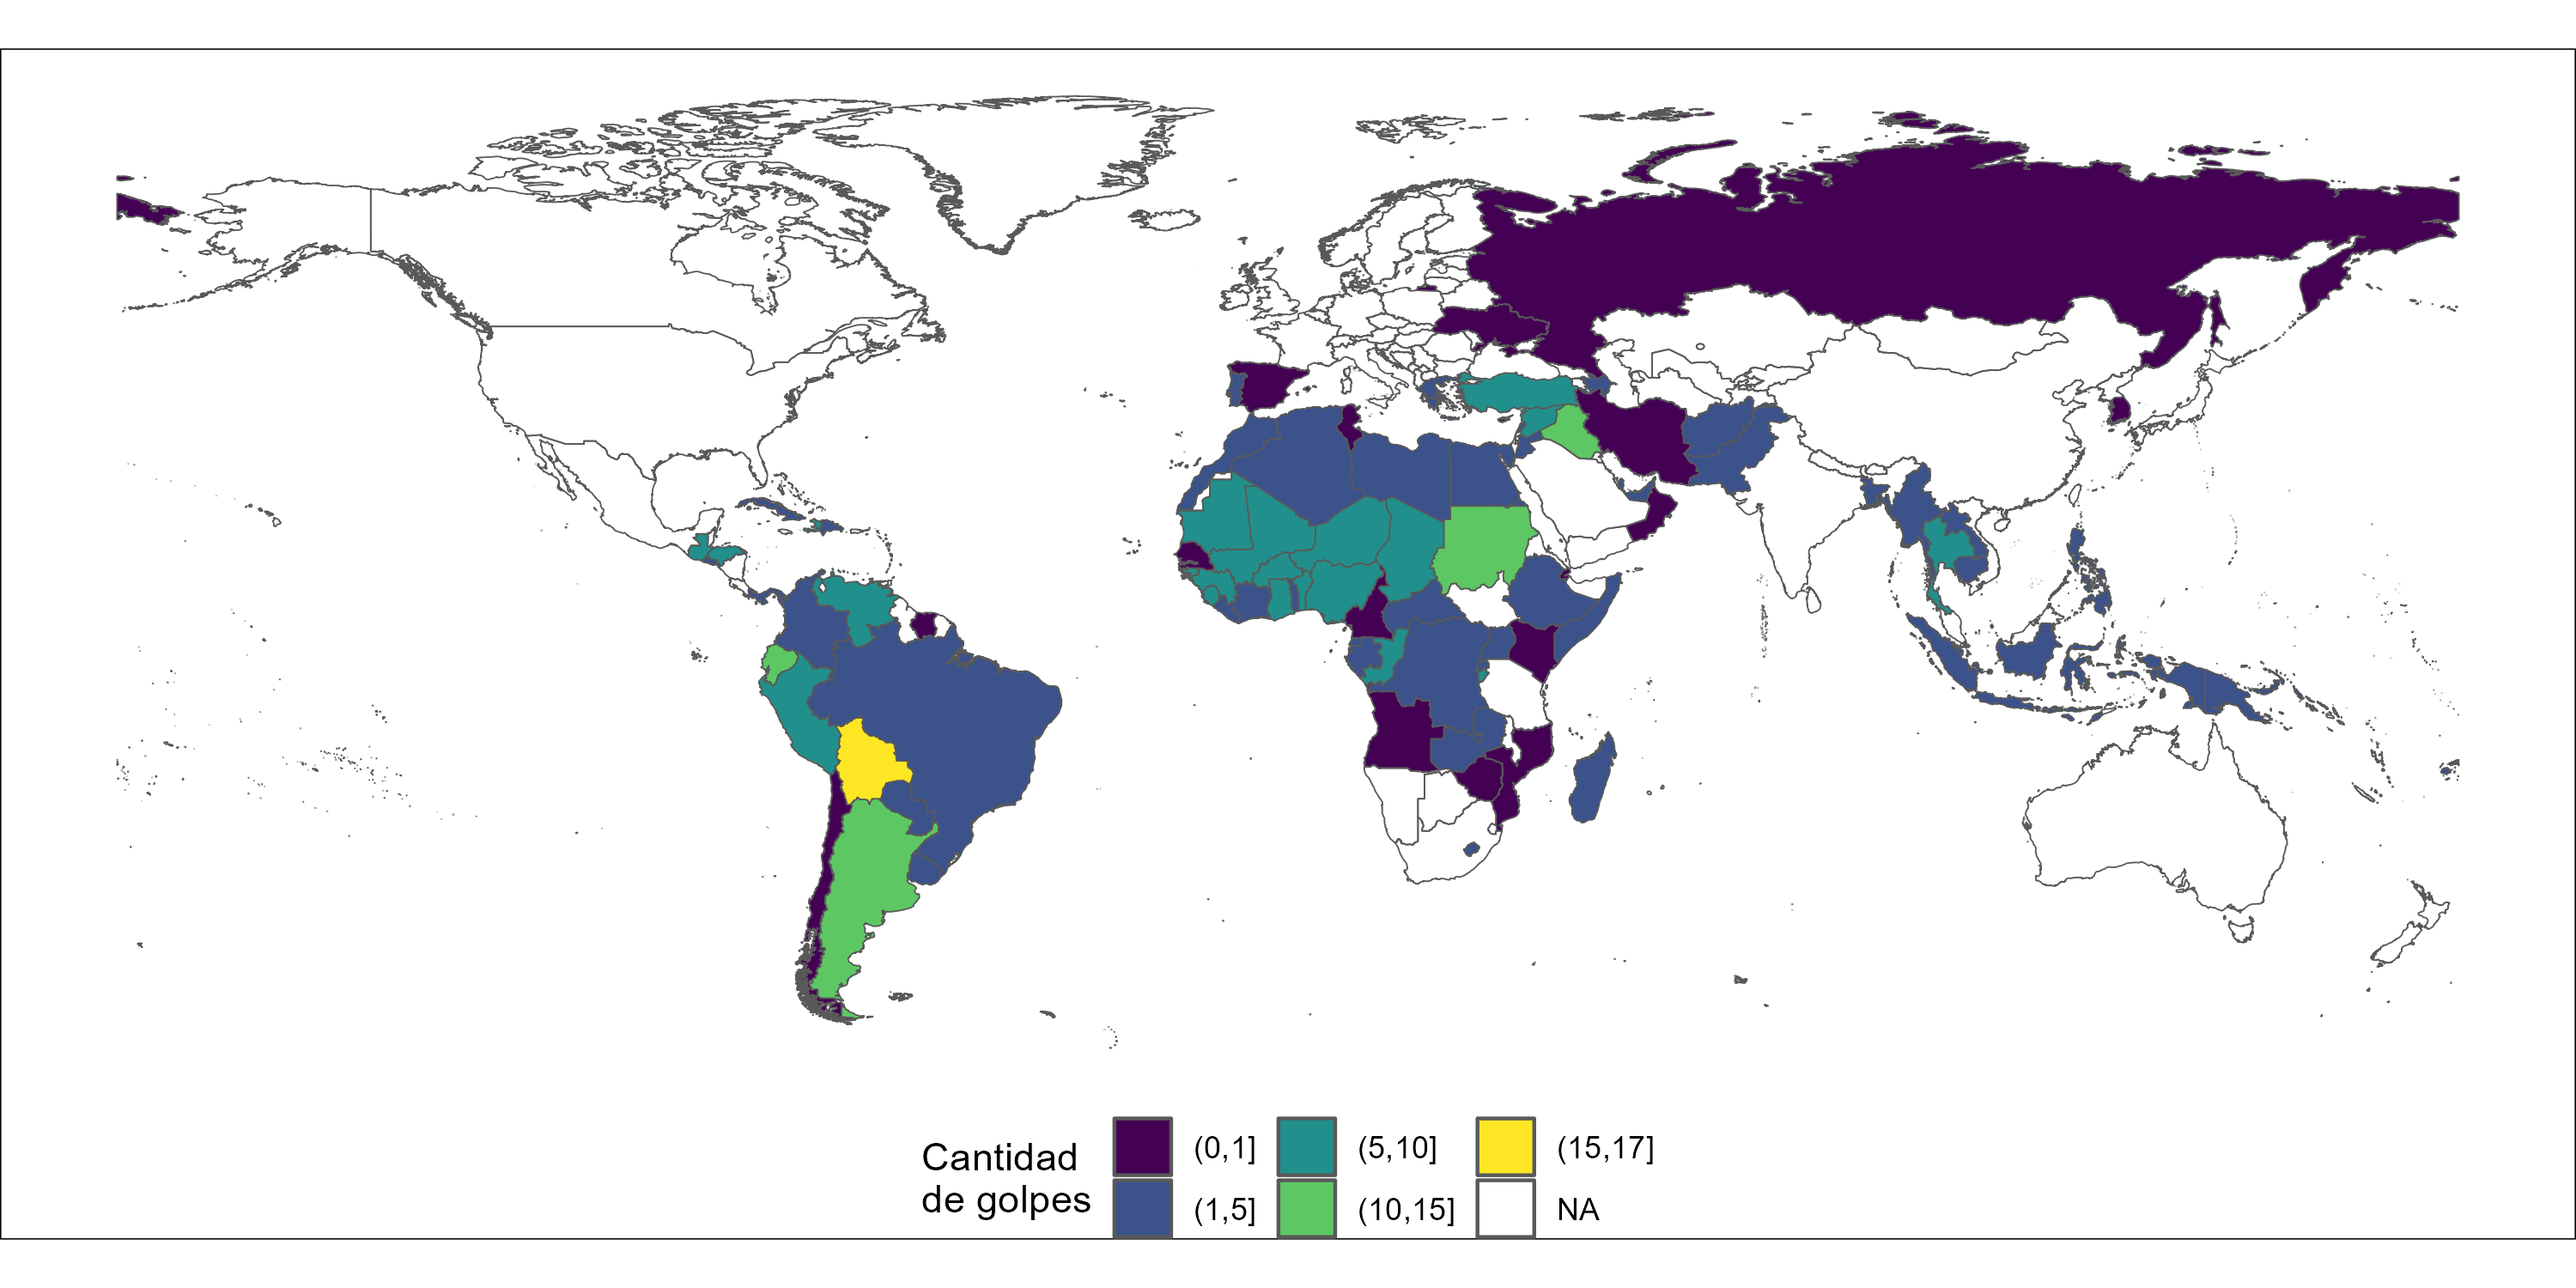
\includegraphics[width=1\textwidth]{2_golpes.png}
  \caption{Golpes de estado período (1950-2023) (\cite{Pow11}) \label{fig::mapa_golpes}}
\end{figure}

Con mayor precisión, observamos que la región del Sahel se destaca con respecto a sus
vecinos africanos. Los países en donde más golpes de estado se han producido son
Bolivia (17), Sudán (14), Argentina (13), Ecuador (11), Iraq (11), Siria(11), 
Guatemala (10) y Tailandia (10).

Desagregando por década se observan algunos cambios, así como la persistencia en 
algunas regiones. La región del Sahel y varias naciones circundantes fueron 
persistentemente afectadas por golpes de estado desde los años 60. En América del 
Sur, en cambio, la presencia casi total de situaciones golpistas en la región se 
fue acotando a partir de los años 80 hasta finalmente desaparecer en el siglo 
xxi. Para observar con más detalle y discriminado por años y países se puede ver 
la figura \ref{fig:golpes_anios}.

\begin{figure}[H]
  \centering  
  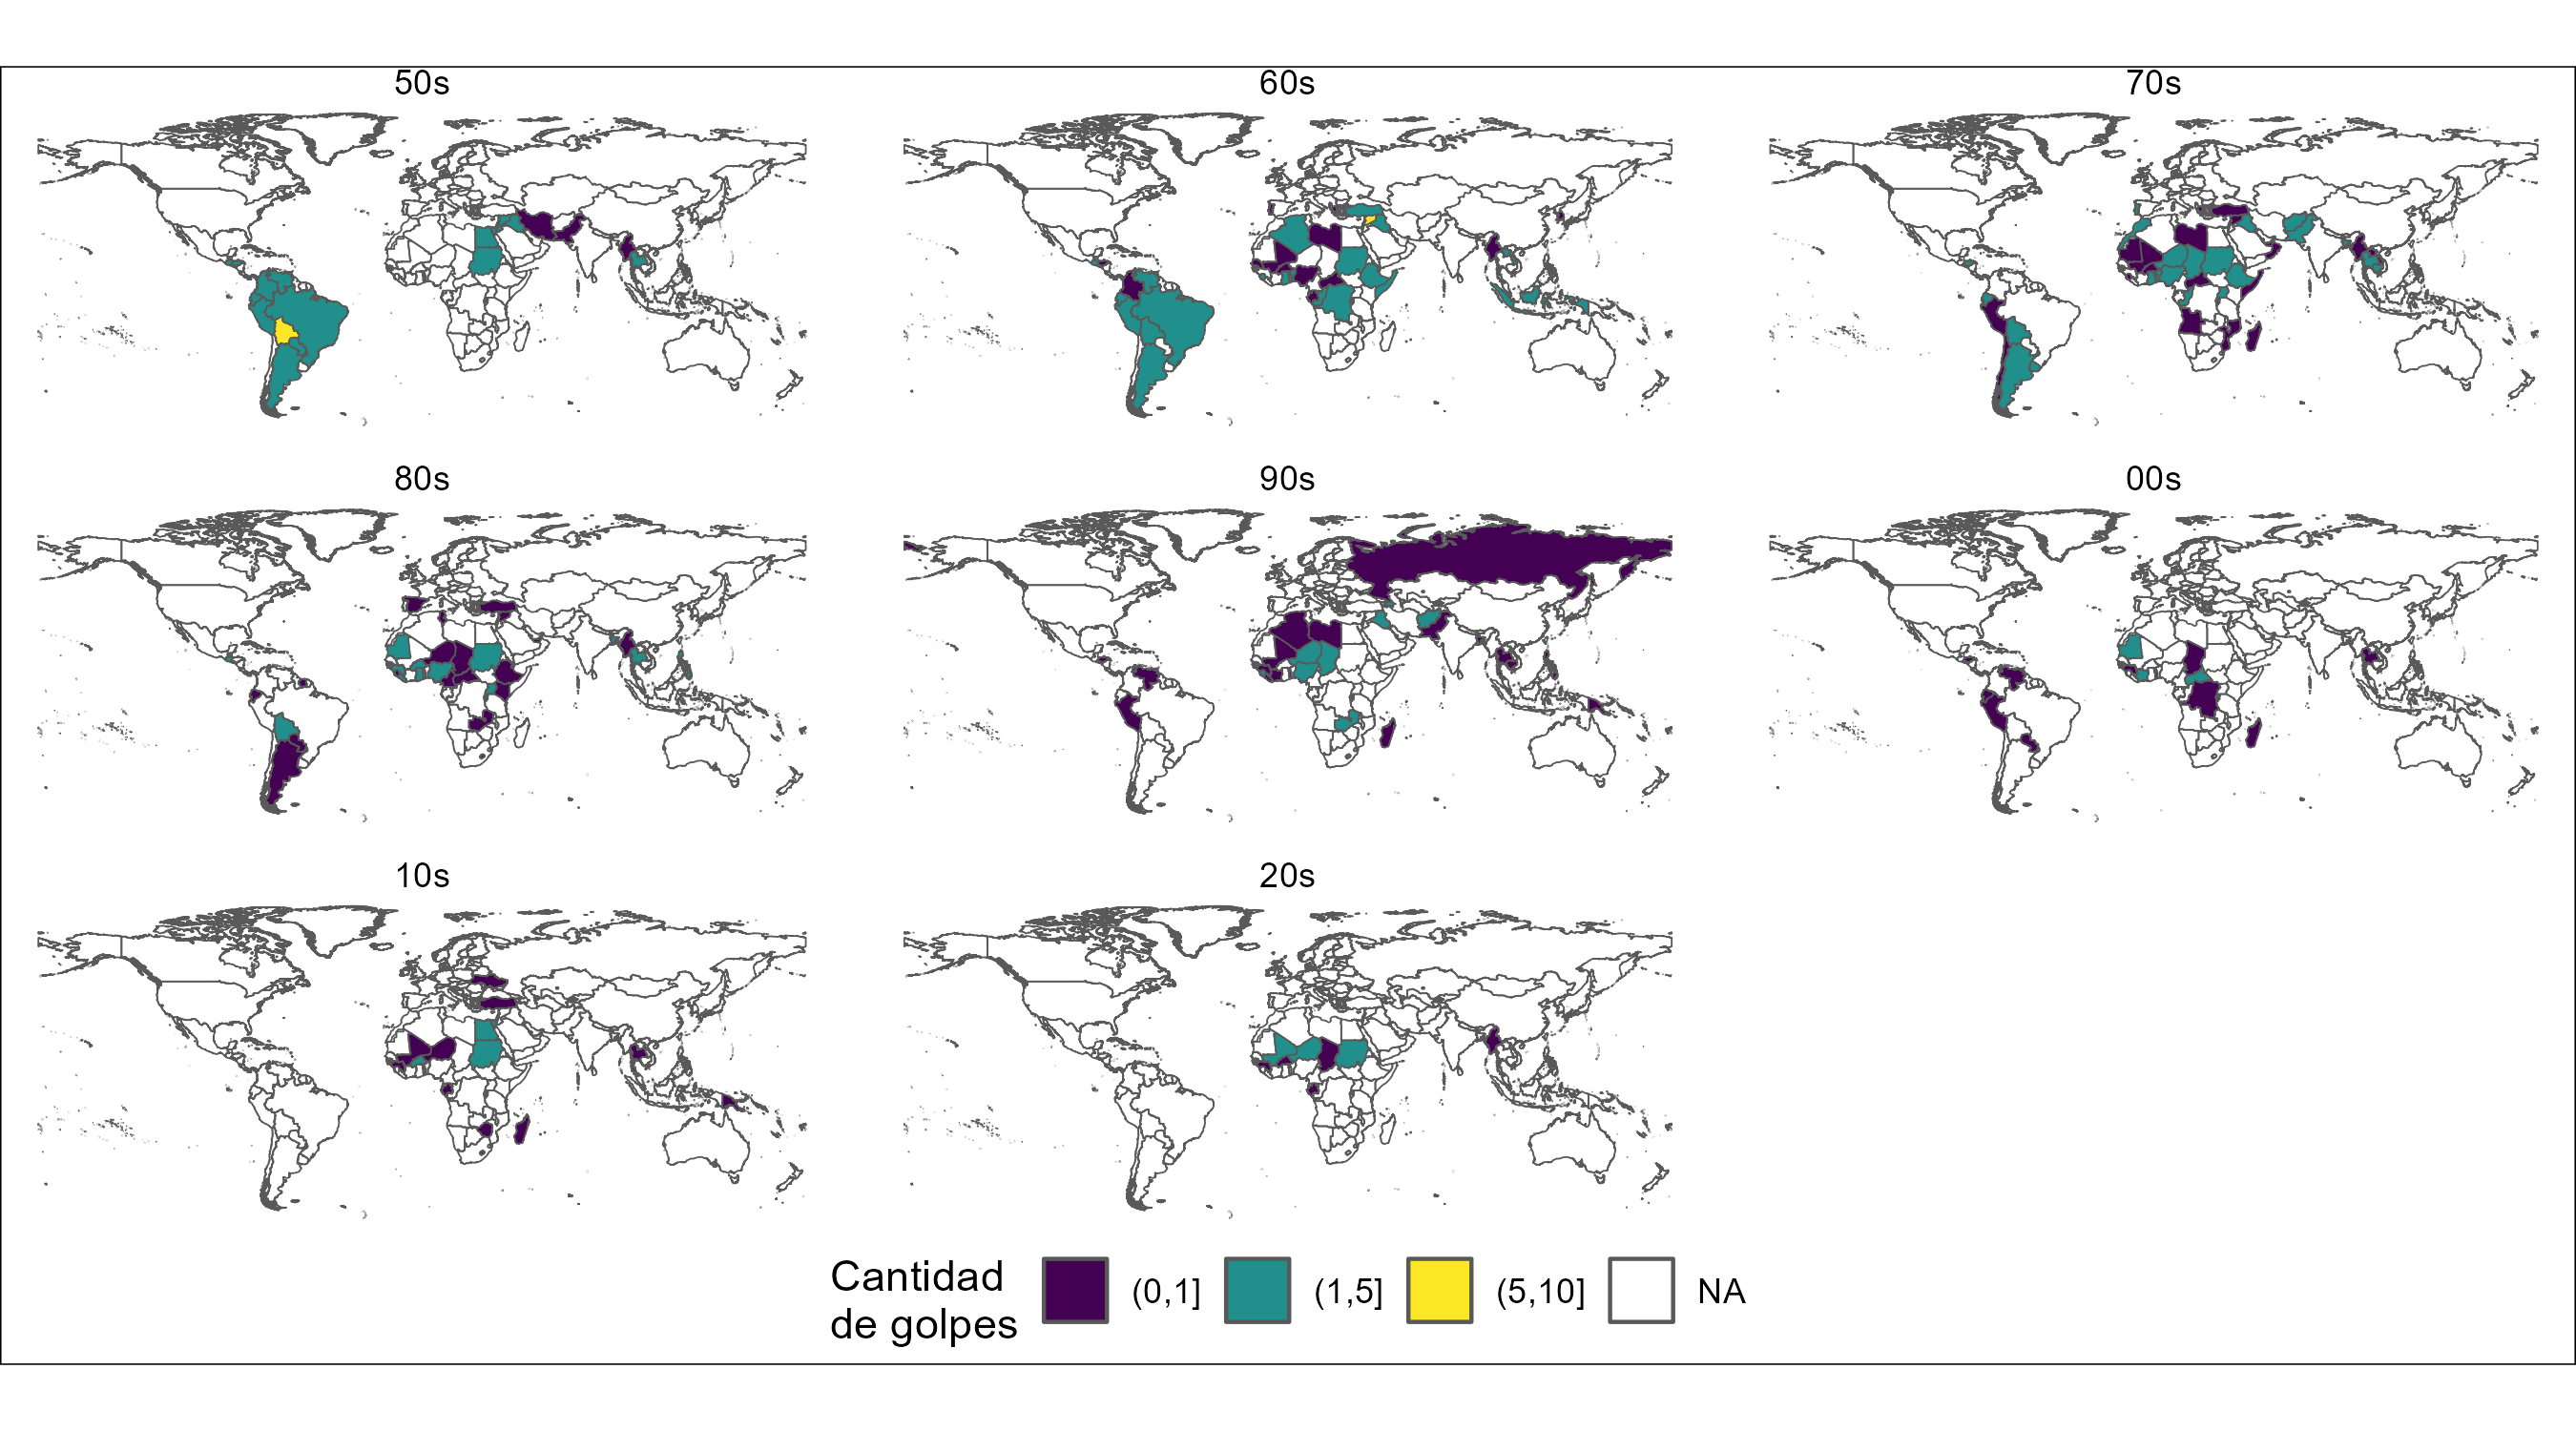
\includegraphics[width=1\textwidth]{3_golpes_decadas.png}
  \caption{Conteo de golpes por década (\cite{Pow11}) \label{fig:golpes_decadas}}
\end{figure}

\section{Resultados y discusión}
En primer lugar, se ralizó la optimización bayesiana de ambos modelos según lo indicado
en la metodología. En el caso de XGBoost se pudo realizar las 100 iteraciones sin mayores
inconvenientes, tomando los valores óptimos de hiperparámetros para el entrenamiento 
final.
Con respecto a Random Forest, en cambio, se alcanzaron 53 iteraciones, debido a que cada
iteración consumía una gran cantidad de tiempo (en promedio una hora) y no se observaban
mejoras significativas en el AUC. De las iteraciones generadas, se tomó los 
hiperparámetros
del segundo mejor AUC, puesto que la diferencia con el ganador en el score era 
insignificante, pero el tiempo de cómputo era menos de la mitad.

Una vez seleccionado los mejores hiperparámetros, se procede a entrenar los modelos en el
conjunto de entrenamiento final, el cual abarca los registros desde 1950 hasta 2019; así
como a evaluar el desempeño del mismo en los años 2020, 2021 y 2022 para emular el trabajo
realizado por el FMI.

Es importante destacar que existen dos enfoques para evaluar el modelo en los años de
testeo: por un lado se pueden evaluar todos los años en su conjunto utilizando como datos
de entrenamiento los registros hasta el año anterior del primer año de validación. Una
opción alternativa es ir entrenando el modelo hasta el año anterior al de validación para
cada año individualmente, de manera de poder utilizar todos los años anteriores y no 
perder
performance. Para este trabajo utilizamos el primer enfoque, es decir que entrenamos los 
modelos hasta 2019 y los evaluamos en todos los años de evaluación a la vez, de manera de
aprehender de manera geenral la importancia de cada variable en la predicción de la
variable objetivo.

En el cuadro \ref{tab:performance} observamos el desempeño de los modelos en los años
de testeo. Por un lado figura el AUC individual de cada año por separado y por el otro
observamos el AUC acumulada es decir, evaluando en ese año junto con los anteriores.

\begin{table}[H]
  \centering
    \begin{tabular}{lcccc}
      \toprule
      & \multicolumn{2}{c}{XGBoost} & \multicolumn{2}{c}{Random Forest} \\
      Año  & AUC      & AUC      & AUC      & AUC  \\
           &          & acumulada&          & acumulada \\
      \midrule
      2020 & 1.000000 & 1.000000 & 1.000000 & 1.000000 \\
      2021 & 0.750000 & 0.785714 & 0.830443 & 0.855718 \\
      2022 & 0.666667 & 0.750000 & 0.666667 & 0.799051 \\
      \bottomrule
    \end{tabular}
  \caption{Performance por año puntual y acumulado de XGBoost y 
  Random Forest\label{tab:performance}}
\end{table}

Lo primero que podemos observar es que ambos modelos logran una performance perfecta 
para el año 2020, lo cual resulta esperable ya que cuentan con información del año 
inmediatamente anterior. También esperable, la performance decae en los años siguientes, 
lo cual también impacta en el valor del AUC acmulada. Lo más destacable es que Random 
Forest logra una mejor performance que XGBoost en el resto de años, alcanzando un AUC de 
casi 0.8 y 0.75, respectivamente. Con esta información, se tomó la decisión de continuar 
el análisis de resultados con Random Forest.


\begin{table}[H]
  \centering
    \begin{tabular}{rllll}
      \toprule
      Año & País & ¿Hubo golpe? & Predicción & Resultado \\
      \midrule
      2020 & Mali                  & Sí & Sí & Verdadero positivo \\
      2021 & Burma/Myanmar         & Sí & Sí & Verdadero positivo \\
      2021 & Sudan                 & Sí & Sí & Verdadero positivo \\
      2021 & Guinea                & Sí & Sí & Verdadero positivo \\
      2021 & Chad                  & Sí & Sí & Verdadero positivo \\
      2022 & Burkina Faso          & Sí & Sí & Verdadero positivo \\
      2021 & Mali                  & Sí & No & Falso negativo \\
      2021 & Niger                 & Sí & No & Falso negativo \\
      2022 & Guinea-Bissau         & Sí & No & Falso negativo \\
      2022 & Sao Tome and Principe & Sí & No & Falso negativo \\
      \bottomrule
    \end{tabular}
  \caption{Falsos negativos y verdaderos positivos (Random Forest) \label{tab:resultados}}
\end{table}

% \begin{table}[H]
%   \centering
%     \begin{tabular}{lrr}
%       \toprule
%       Descripción & Variable & Importancia & Importancia acumulada \\
%       \midrule
%       Días desde comienzo del régimen       & v2regdur                  & 0.131 & 0.131 \\
%       ¿El régimen terminó por un golpe      &                           &          &          \\
%       de estado (año anterior)              & v2regendtypems\_0\_lag\_1 & 0.110 & 0.241 \\
%       ¿El ejecutivo es electo?              & v2x\_hosinter             & 0.106 & 0.347 \\
%       ¿Legislatura cerrada o abortada?      & v2xlg\_leginter           & 0.067 & 0.415 \\
%       Proceso más importante para terminar  &                           &          &          \\
%       con un régimen (año anterior)         & v2regendtype\_lag\_1  & 0.055 & 0.470 \\
%       Influencia de las FFAA sobre el       &                           &          &          \\
%       Poder Ejecutivo                       & v2x\_ex\_military         & 0.042 & 0.512 \\
%       FFA se movilizan contra el régimen?   & v2regoppgroupsact\_5      & 0.019 & 0.531 \\
%       ¿golpes de estado en el último año?   & coup\_lag\_1              & 0.008 & 0.539 \\
%       Influencia de las FFAA sobre el       &   &   &   \\
%       Poder Ejecutivo (año anterior)        & v2x\_ex\_military\_lag\_1 & 0.006 & 0.545 \\
%       ¿Cómo llega el jefe de estado al gob? & v2expathhs                & 0.004 & 0.549 \\
%       \bottomrule
%     \end{tabular}
%   \caption{Importancia de las variables (Random Forest) \label{tab:feat_imp}}
% \end{table}


\section{Anexo}

\begin{figure}[H]
  \centering  
  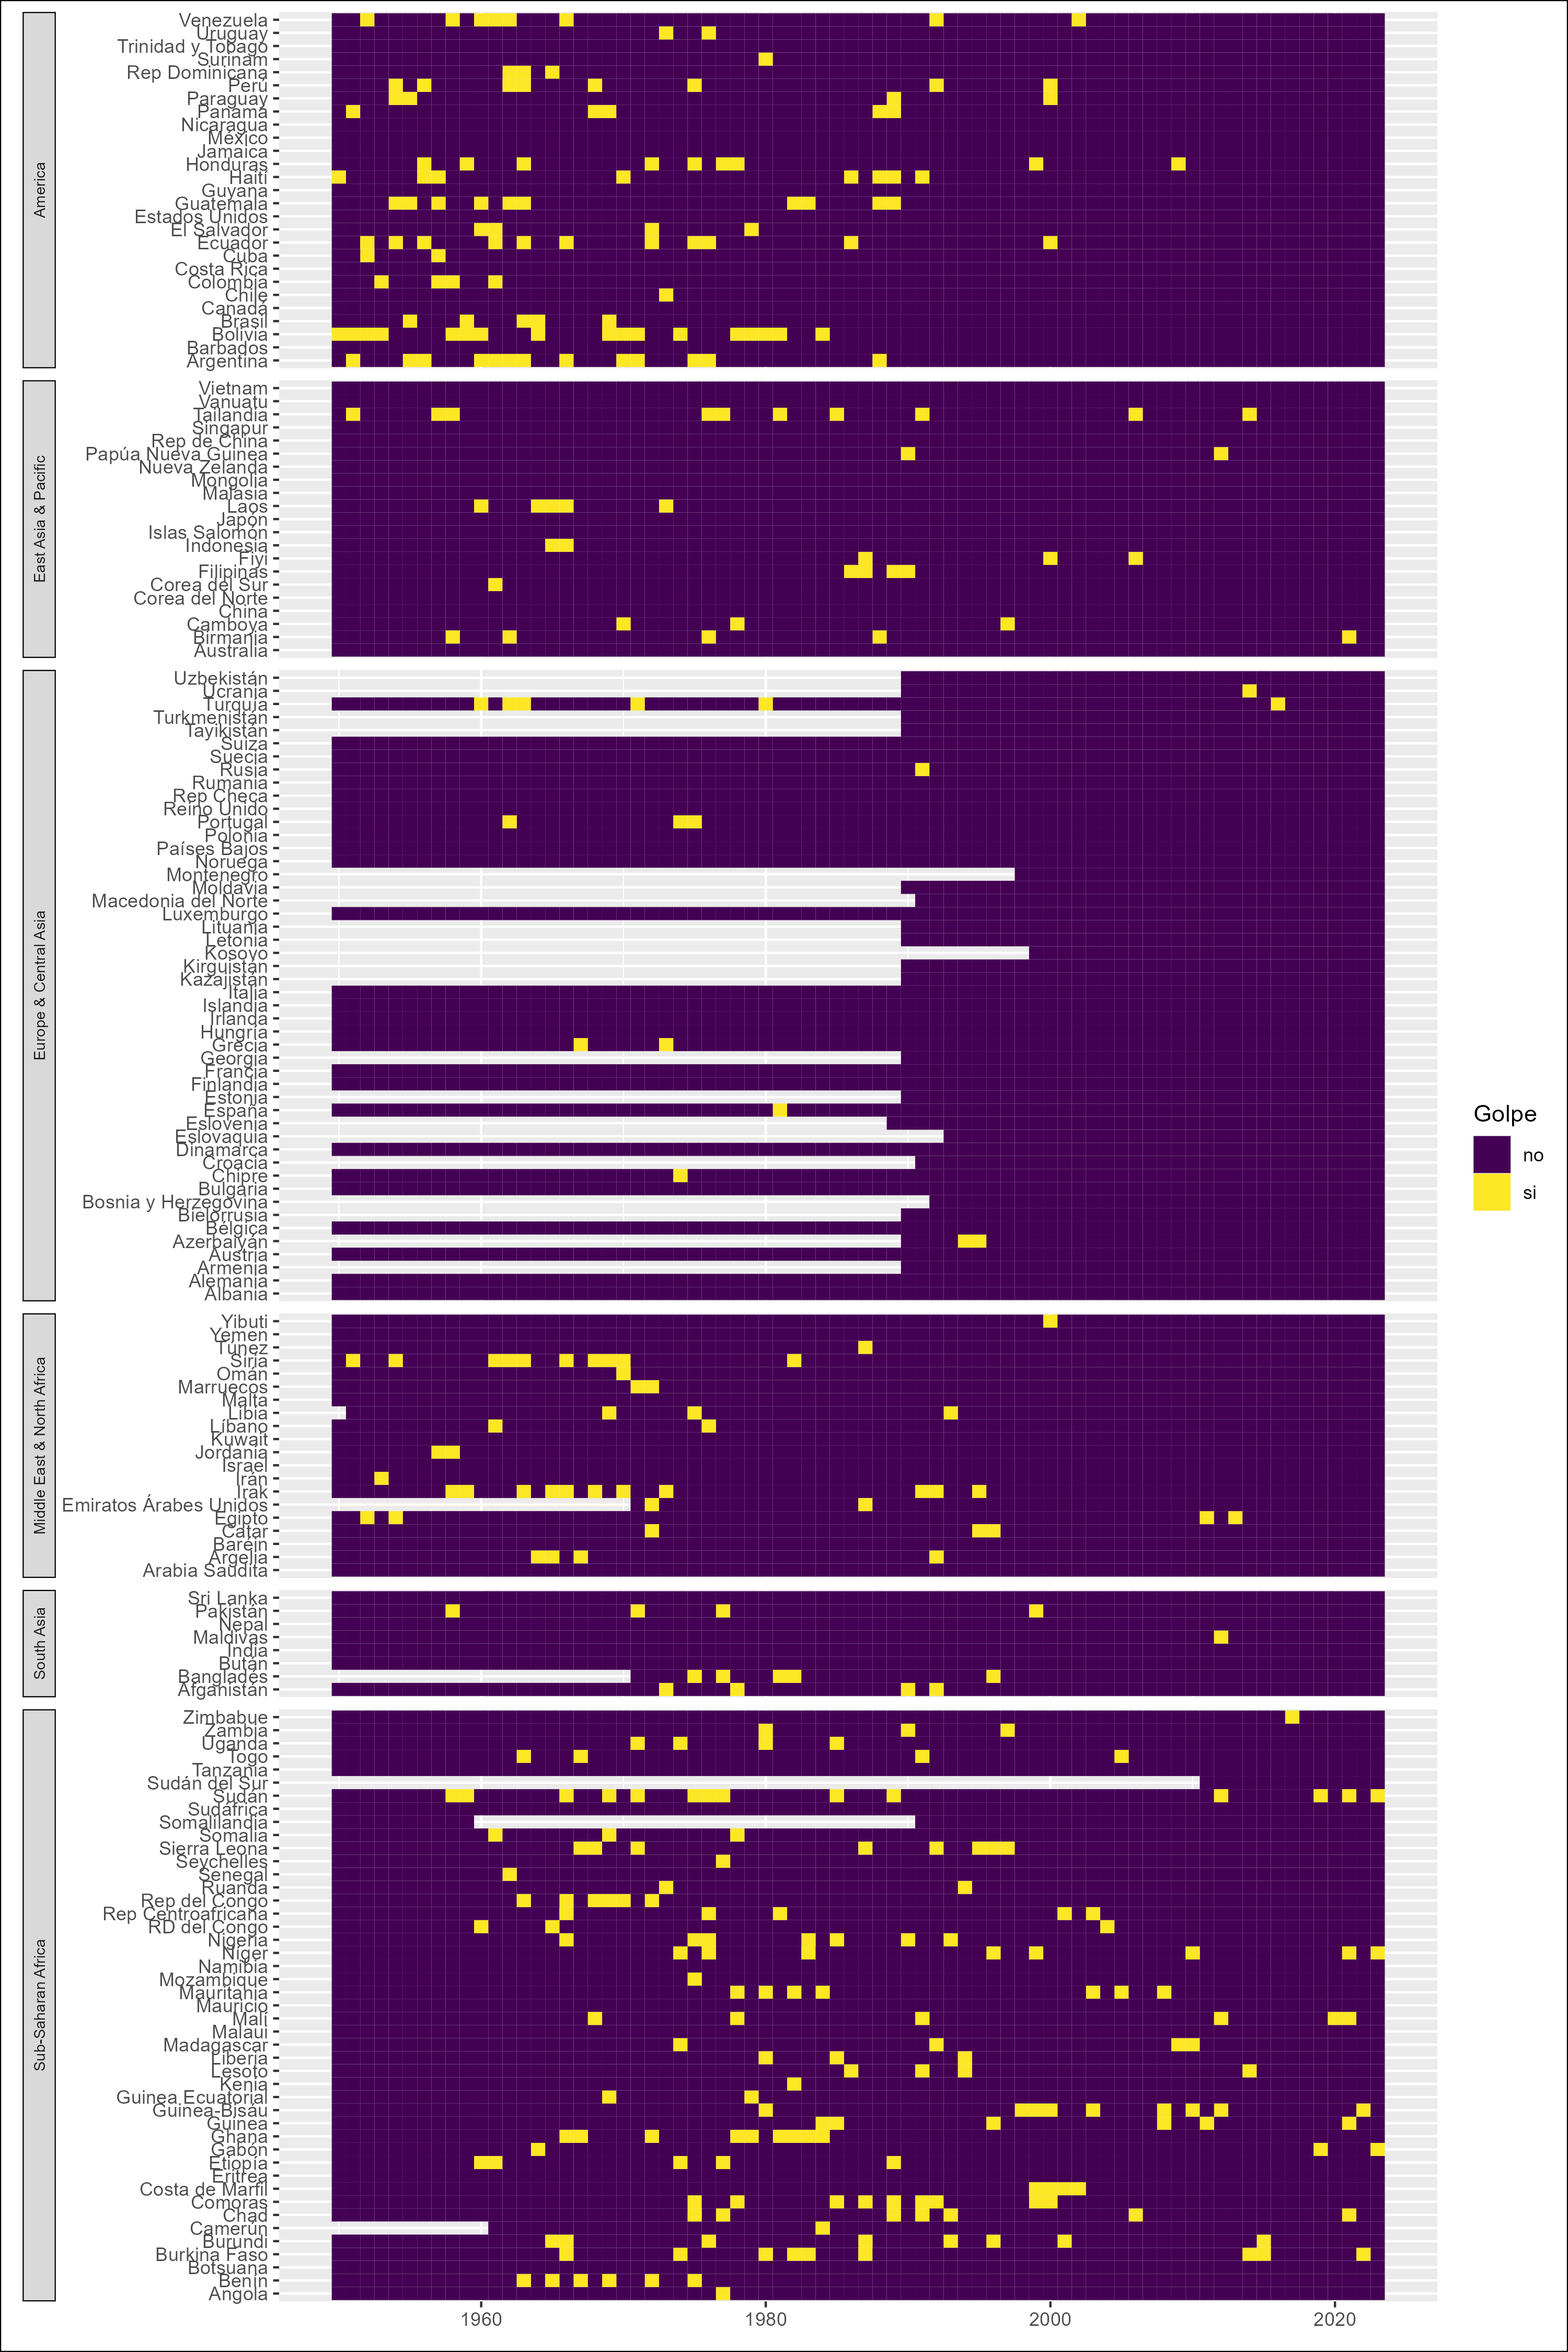
\includegraphics[width=1\textwidth]{4_golpes_anios.png}
  \caption{Conteo de golpes por año y región (\cite{Pow11})\label{fig:golpes_anios}}
\end{figure}

\printbibliography

\end{document}